%%%%%%%%%%%%%%%%%%%%%%%%%%%%%%%%%%%%%%%%%%%%%%%%%%%%%%%%%%%%%%%%%%%%%%%%%%%%%%%%
% b-tree.tex
% An example demonstrating how to create a B-tree in LaTeX with TikZ
% https://github.com/mhyee/latex-examples/
%%%%%%%%%%%%%%%%%%%%%%%%%%%%%%%%%%%%%%%%%%%%%%%%%%%%%%%%%%%%%%%%%%%%%%%%%%%%%%%%


% LaTeX Preamble
% Load packages and set options as needed
%%%%%%%%%%%%%%%%%%%%%%%%%%%%%%%%%%%%%%%%%%%%%%%%%%%%%%%%%%%%%%%%%%%%%%%%%%%%%%%%

% Set the document class to "article"
% Pass it "12pt" and "letterpaper" options
\documentclass[12pt,letterpaper]{article}

% We don't need the special font encodings, but still
% good practice to include these. See:
%
% http://tex.stackexchange.com/questions/664/why-should-i-use-usepackaget1fontenc
% http://dsanta.users.ch/resources/type1.html
\usepackage[T1]{fontenc}
\usepackage{ae,aecompl}
% http://tex.stackexchange.com/a/44699
% http://tex.stackexchange.com/a/44701
\usepackage[utf8]{inputenc}

% Use Latin Modern, an improved version of the Computer Modern font
\usepackage{lmodern}

% TikZ is what lets us draw graphics
\usepackage{tikz}

% Disable page numbering
\pagestyle{empty}

% Decrease the table column spacing
% We're using tables to represent nodes in this example
\setlength{\tabcolsep}{2pt}

% Define our own macros, for convenience
%%%%%%%%%%%%%%%%%%%%%%%%%%%%%%%%%%%%%%%%%%%%%%%%%%%%%%%%%%%%%%%%%%%%%%%%%%%%%%%%

% \ensuremath{ARG} is used to enable mathematics mode in a macro
% ARG will always be rendered in math mode,
% regardless of which mode the macro is called in
%
% http://www.giss.nasa.gov/tools/latex/ensuremath.html

% These macros create single-row table with the arguments as values
% Each value is centred, and all borders are drawn
% eg \threenode{a}{b}{c} creates a single-row table with cols a, b, c

\newcommand{\onenode}[1]{%
  \begin{tabular}{|c|}
    \hline #1\\ \hline
  \end{tabular}
}
\newcommand{\twonode}[2]{%
  \begin{tabular}{|c|c|}
    \hline #1 & #2\\ \hline
  \end{tabular}
}
\newcommand{\threenode}[3]{%
  \begin{tabular}{|c|c|c|}
    \hline #1 & #2 & #3\\ \hline
  \end{tabular}
}
\newcommand{\fournode}[4]{%
  \begin{tabular}{|c|c|c|c|}
    \hline #1 & #2 & #3 & #4\\ \hline
  \end{tabular}
}
\newcommand{\fivenode}[5]{%
  \begin{tabular}{|c|c|c|c|c|}
    \hline #1 & #2 & #3 & #4 & #5\\ \hline
  \end{tabular}
}

% Begin the actual typesetting, by starting the "document" environment
%%%%%%%%%%%%%%%%%%%%%%%%%%%%%%%%%%%%%%%%%%%%%%%%%%%%%%%%%%%%%%%%%%%%%%%%%%%%%%%%
\begin{document}

% This is a B-tree of minsize 2 (ie order 5), ie
% - each node contains at most 4 KVPs
% - each node has at most 5 children
% - each non-root node contains at least 2 KVPs

% 3 has just been inserted, causing an overflow
% The tree looks something like this
%
%                             51
%                12 46                     62 91
% 1 2 3 5 7  38 42 43 45  47 48     53 55  68 78  92 93 97

  \begin{center}
    % Set the options for the diagram
    % - set the distance between each level
    % - set a style for every node
    % - "bad" nodes have a 50% opaque red filling
    % - set the distances between siblings of level 1 and level 2
    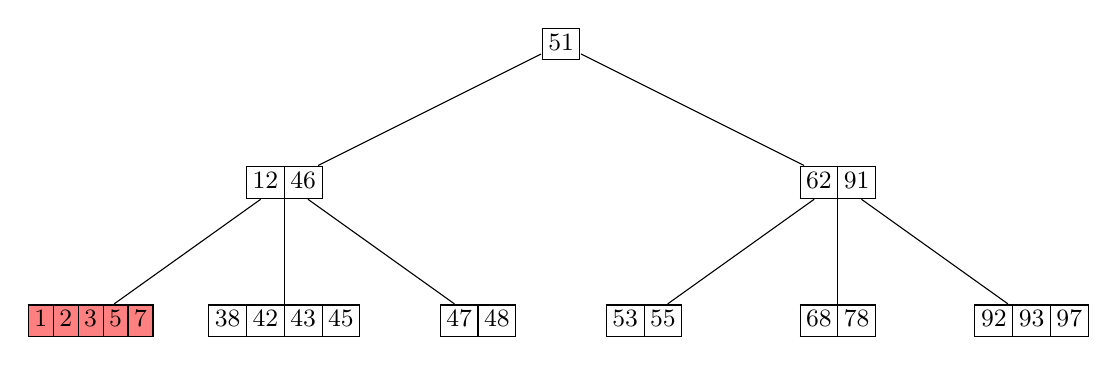
\begin{tikzpicture}[
      level distance=50pt,
      every node/.style={inner sep=0pt,font=\small},
      bad/.style={fill=red!50},
      level 1/.style={sibling distance=200pt},
      level 2/.style={sibling distance=70pt}
    ]

      % Draw the nodes, filling in their values and children
      \node {\onenode{51}}
        child {node {\twonode{12}{46}}
          % This node is bad (too many values), so colour it red
          child {node[bad] {\fivenode{1}{2}{3}{5}{7}}}
          child {node {\fournode{38}{42}{43}{45}}}
          child {node {\twonode{47}{48}}}
        }
        child {node {\twonode{62}{91}}
          child {node {\twonode{53}{55}}}
          child {node {\twonode{68}{78}}}
          child {node {\threenode{92}{93}{97}}}
        }
      ;
    \end{tikzpicture}
  \end{center}

\end{document}

